\section{Integration von CSV-Tools in Jenkins}
\label{sec:Integration}

Ich bin nach mehr als 10h mit fast 150 Jenkins builds, wobei fast alle eine unterschiedliche Konfiguration haben, leider auf keinen positiven Build des Projekts gekommen. Es ist für mich nicht erklärbar und auch Google hilft nicht mehr weiter. Ich habe die einzelnen Steps des Tutorials 1:1 nachgemacht (selsbtverständlich für das Projekt angepasst) und es kommen keine positiven Resultate. Ich habe dann versucht das Shellskript selber zu schreiben und auch ekien Resultate erhalten. Beispielsweise dachte ich, dass es ein Problem zwischen den synced folder gibt, hab es mit chmod versucht, und nichts ist passiert. Ich habe versucht das Projekt von GitHub zu klonen und habe die selben resultate bekommen. 

Hier ist der Output der Jenkins Build Error Console des letzten Builds. Man beachte, dass ein chmod durchgeführt wird, es aber trotzdem einen Permission Error gibt.

\begin{figure}[h!]
	\caption{Jenkins Console Error}
	\centering
	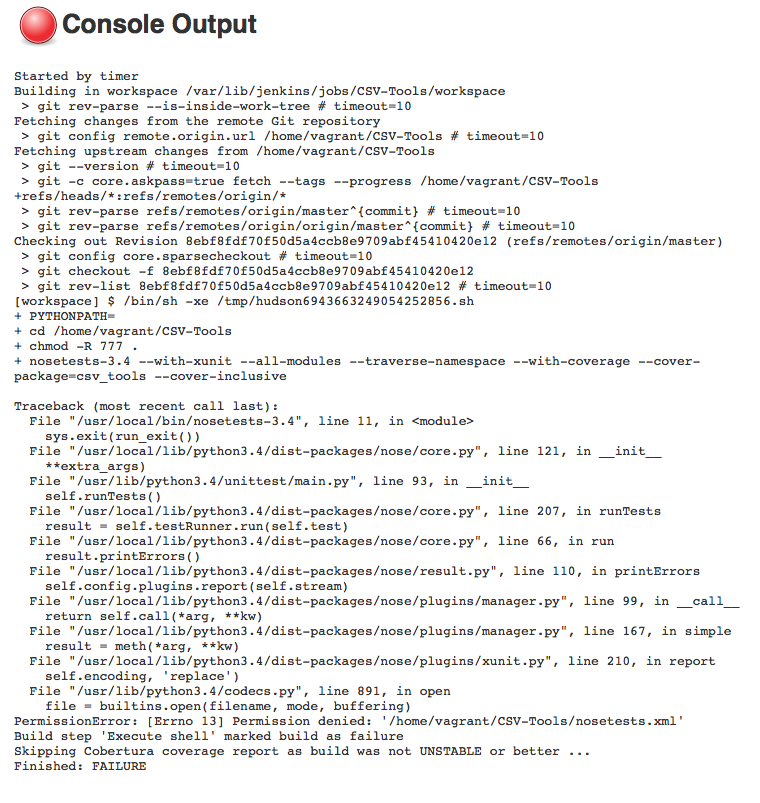
\includegraphics[width=\textwidth]{images/jenkins_consoleError.png}
\end{figure}

Führe ich aber das Buildskript 1:1 zu aus wie ich es konfiguriert habe, bekomm ich alle benötigten files ohne jegliche error meldungen zurück.

\begin{figure}[h!]
	\caption{Jenkins Buld script}
	\centering
	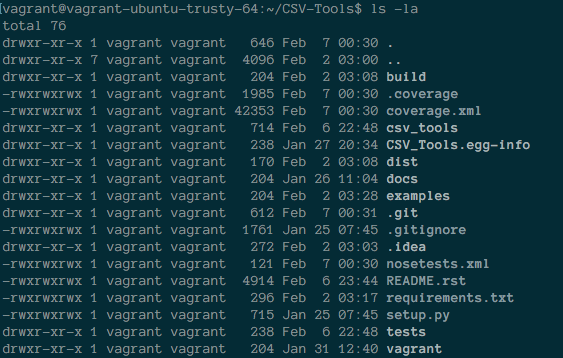
\includegraphics[width=\textwidth]{images/vagrant_script.png}
\end{figure}

Es ergibt für mich einfach keinen Sinn mehr.
